% Lecture Template for ME3050-001-002-Tristan Hill - Spring 2020
% Dynamics Modeling and Controls
% Time Response - Lecture 1

% I am finally converting my stuff to BEAMER

% Document settings

%\documentclass{beamer}                  % for presentation ?
\documentclass[handout]{beamer}  % for handout ?
\usepackage{beamerthemesplit}
\usepackage{amsmath}
\usepackage{listings}
\usepackage{multicol}

\beamertemplateballitem

\definecolor{TTUpurple}{rgb}{0.3098, 0.1607, 0.5176} % TTU Purple (primary)
\definecolor{TTUgold}{rgb}{1.0000, 0.8666, 0.0000} % TTU Gold (primary)

\setbeamercolor{palette primary}{bg=TTUpurple,fg=TTUgold}
\setbeamercolor{palette secondary}{bg=black,fg=TTUgold}
\setbeamercolor{palette tertiary}{bg=black,fg=TTUpurple}
\setbeamercolor{palette quaternary}{bg=TTUgold,fg=black}
\setbeamercolor{structure}{fg=TTUpurple} % itemize, enumerate, etc
\setbeamercolor{section in toc}{fg=TTUpurple} % TOC sections

%\usefonttheme{professionalfonts}

\newcommand{\LNUM}{1\hspace{2mm}} % Lecture Number 

\newcommand{\Lagr}{\mathcal{L}} % lagrangian

\newcommand{\vspcc}{\vspace{6mm}\\ } 
\newcommand{\vspc}{\vspace{3mm}\\ } 
\newcommand{\hspc}{\hspace{5mm} } 

\newcommand{\secondtitle}{Time Response of First Order Systems}% second line of the title of this presentation , aka the topic of this lecture

\title{Time Response - Lecture \LNUM}
\author{ME3050 - Dynamics Modeling and Controls} % original formatting from Mike Renfro, September 21, 2004

\date{March 29, 2020}

\begin{document}

\lstset{language=MATLAB,basicstyle=\ttfamily\small,showstringspaces=false}

% Section 0: Outline
\frame{\titlepage \center\textbf{\secondtitle}\vspace{5mm}\\}

\frame{

\large \textbf{Lecture \LNUM - \secondtitle} \vspace{3mm}\\

%Topics : \vspace{3mm}\\ % ' topics' are beamer 'sections' - TWH

 \begin{itemize}
	\item Welcome Back!\vspace{3mm}\\ % Section 1
	\item Free Response of a First Order Model\vspace{3mm}\\% Section 2
	\item Stability in Dynamic Systems \vspace{3mm}\\ %Section 3
	\item Forced Response of a First Order Model\vspace{3mm}\\ % Section 4
	%\item Example\vspace{3mm}\\ % Section 5 - 5 is almost too many...
\end{itemize}
}

% Section 1: Welcome Back!
\section{Welcome Back!}
\subsection{Welcome to New Video Lectures }

\frame{

  \frametitle{Welcome to New Video Lectures}
  \large{\it Welcome Back!\vspace{3mm}\\}

\begin{itemize}
\item Things are going to be different but we will still learn! \vspace{3mm}\\
\item These new outlines should help keep me/us on track.  \vspace{3mm}\\
\item The material will be organized in 20-30 min videos, and you can watch them at anytime. \vspace{3mm}\\
\end{itemize}

}

\subsection{Welcome to Chapter 8 -  {\it Time Response} }

\frame{

  \frametitle{Welcome to Chapter 8 -  {\it Time Response}}

  \large{Chapter 8 - System Analysis in the Time Domain} \vspc	

  We have jumped forward a bit into chapter 8 but that is ok. We will go back into Ch6/7 when soon. \vspace{3mm}\\

}

% Section 2: Free Response of a Moving Mass - first order model
\section{Free Response of a First Order Model}
\subsection{Model and EOM}

\frame{
  
  \frametitle{Model and EOM}

Consider the model of the moving mass we derived. \vspace{3mm}\\

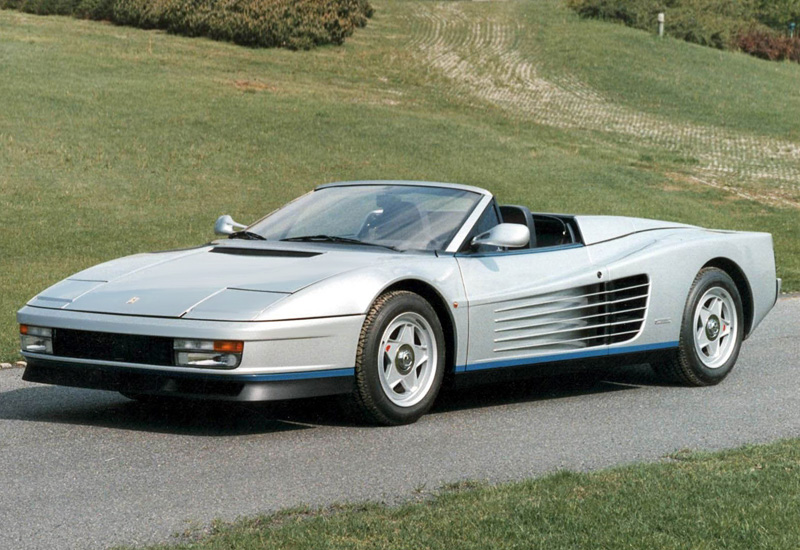
\includegraphics[scale=.15]{ferrari.jpg} \vspace{3mm}\\

\large The EOM is:\vspace{3mm}\\

\scalebox{1.5}{$m\dot{v} +cv=0$} \vspace{3mm}\\

}

\subsection{Solution with Laplace Transforms Method} 

\frame{
  
  \frametitle{Solution with Laplace Transforms Method}

%\textbf{ \Large Solve for $v(t)$ using a method of your choice. \\\\ }\\

%\textbf{\large The method of Laplace Transforms is shown.}\\\\

	\scalebox{1.25}{$\Lagr{\{m\dot{v} +cv}=0\}$ $ \implies$  $m [sV(s) -v(0) ] +cV(s)=0$}  \vspace{3mm}\\

	\scalebox{1.25}{$(ms+c)V(s)=\frac{mv(0)}{(ms+c)} = \frac{V(0)}{s+\frac{c}{m}}$} \vspace{8mm}\\

\large We can find the expected result from the table. \vspace{5mm}\\

	\scalebox{1.25}{$v(t)=v(0)e^{-\frac{c}{m}t} = v(0)e^{-\frac{t}{\tau}} $ \hspace{5mm} with \hspace{5mm}$\tau = $}

}

\subsection{Sketch Response Equation} 

\frame{
  
  \frametitle{Sketch Response Equation}

\large Sketch the System Response in the time Domain.  \vspace{3mm}\\

\scalebox{1.25}{$v(t)=v(0)e^{-\frac{t}{\tau}} $ }  \vspace{3mm}\\

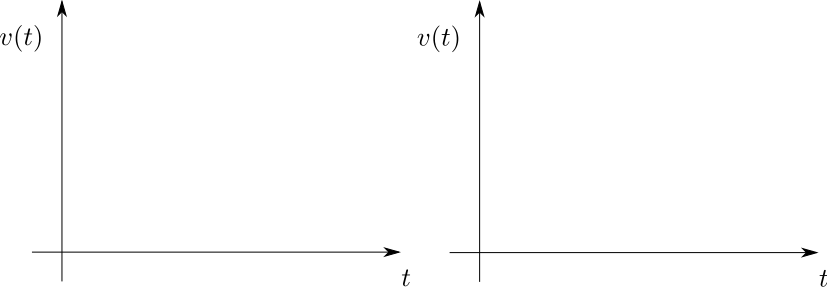
\includegraphics[scale=0.5]{lecture1_fig1.png} \\

\large Is this a stable system? What does that mean?\\

}

% Section 3: Stability in Dynamic Systems
\section{Stability in Dynamic Systems}

\frame{
  
\frametitle{Stability in Dynamic Systems}

A dynamic system is stable if ...  \vspace{50mm}\\

}


% Section 4: Forced Response of a First Order Model
\section{Forced Response of a First Order Model}
\subsection{Step Input Function} 
\frame{
  
\frametitle{Step Input Function}

\Large Consider the model subject to a Step Input, $f(t)$. \vspace{3mm}\\
\begin{multicols}{2}
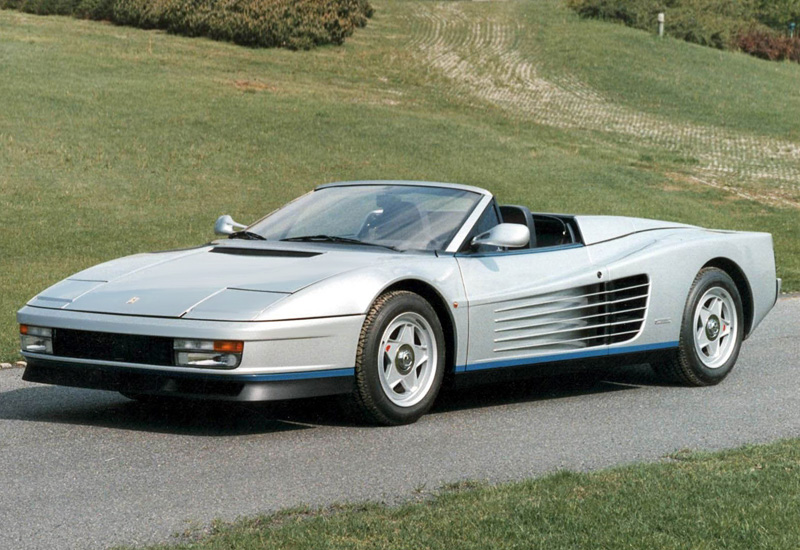
\includegraphics[scale=.15]{ferrari.jpg}  

\scalebox{1.25}{$m\dot{v} +cv=f(t)$} 

\[f(t) = \begin{cases} 
      0 & t < 0 \\
      F & t\geq 0 \\
   \end{cases}
\]\\

\end{multicols}

}

\subsection{Solution with Laplace Transforms Method} 
\frame{

  
\frametitle{Solution with Laplace Transforms Method - Step 1}

\large The method of Laplace Transforms is shown. \vspace{5mm} \\

	\scalebox{1.15}{$\Lagr{\{m\dot{v} +cv}=F\}$ $ \implies$  $m [sV(s) -v(0) ] +cV(s)=\frac{F}{c}$}  \vspace{0mm} \\

	\scalebox{1.15}{$(ms+c)V(s)=\frac{F}{s}+mv(0)$}  \vspace{5mm} \\

\large Solve for $V(s)$. \vspace{2mm} \\
	\scalebox{1.15}{$V(s)=\frac{F}{s(ms+c)}+\frac{mv(0)}{ms+c}$} 

}

\frame{

\frametitle{Solution with Laplace Transforms Method - Step 2}

Expand $V(s) $as a partial fraction. \vspace{2mm} \\
	\scalebox{1.15}{$V(s)=\frac{F}{s(ms+c)}+\frac{mv(0)}{ms+c}\implies \frac{F}{s(ms+c)}=\frac{a}{s} +\frac{b}{ms+c}$} \vspace{5mm} \\
\large 'Cover up' to find the coefficients. \vspace{2mm} \\

	\scalebox{1.15}{$a=\frac{F}{m\times0+c} $ \hspace{5mm} and \hspace{5mm} $b=\frac{F}{\frac{-c}{m}}=\frac{-Fm}{c}$}  \vspace{2mm} \\

\large This leads to a form that can be inverted with the table. \vspace{5mm} \\

\scalebox{1.15}{$V(s)=\frac{F}{c}\{ \frac{1}{s}-\frac{1}{s+\frac{c}{m}}\}+\frac{v(0)}{s+\frac{c}{m}}$} 

}

\frame{

\frametitle{Solution with Laplace Transforms Method - Step 3}

Can you find these terms in the Table of Laplace Transforms? \vspace{5mm}\\
\scalebox{1.15}{$V(s)=\frac{F}{c}\{ \frac{1}{s}-\frac{1}{s+\frac{c}{m}}\}+\frac{v(0)}{s+\frac{c}{m}}$}  \vspace{5mm} \\

The inverse Laplace transform of $V(s)$ gives the time response. \vspace{5mm}\\

\scalebox{1.15}{$v(t)=\frac{F}{C}\{1-e^{-\frac{t}{\tau}} \} + v(0)e^{-\frac{t}{\tau}} = \{v(0)-\frac{F}{c}\}e^{-\frac{t}{\tau}} + \frac{F}{c}$  }

}



\subsection{Sketch Response Equation}
\frame{

\frametitle{Sketch Response Equation}

\large Sketch the System Response in the time Domain.  \vspace{3mm}\\

\scalebox{1.25}{$v(t)=\{v(0)-\frac{F}{c}\}e^{-\frac{t}{\tau}} + \frac{F}{c}$ }  \vspace{3mm}\\

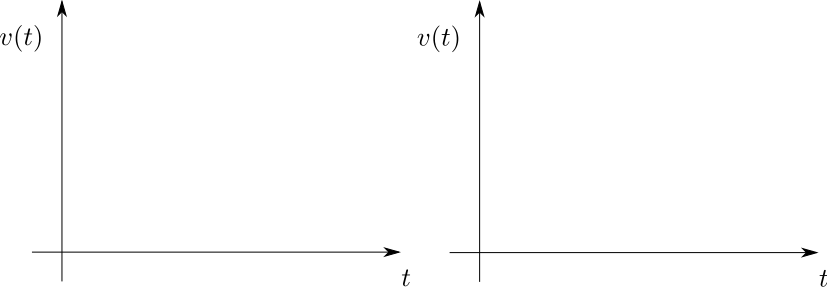
\includegraphics[scale=0.5]{lecture1_fig1.png} \\

\large Is this a stable system?\\

}


\subsection{Components of the Response}
\frame{ 

\frametitle{Components of the Response}

\large In these forms we can see the different components of the response.\vspace{3mm}\\

\scalebox{1.15}{$v(t)=\frac{F}{C}\{1-e^{-\frac{t}{\tau}} \} + v(0)e^{-\frac{t}{\tau}} = \{v(0)-\frac{F}{c}\}e^{-\frac{t}{\tau}} + \frac{F}{c}$  } \vspace{3mm}\\


\large
\begin{itemize}

\item Forced Response\\

\item Free Response\\

\item Transient Response\\

\item Steady-State Response

\end{itemize}


}


% references is not a section for now, for looks and it would be a waste of space
\frame{

\frametitle{References}

\begin{itemize}
	\item System Dynamics, Palm III, Third Edition - Section 8.1 - Response of First Order Systems - pg. 475
\end{itemize}

}
\end{document}









